\section{Описание контейнера}

\paragraph{Линейный односвязный список.}

Линейный односвязный список – это динамическая упорядоченная структура данных, состоящая из элементов одного типа. Каждый элемент содержит основное поле-указатель на объект и поле с указателем на следующий элемент. Элементы не всегда расположены в памяти последовательно.

Преимуществом линейного односвязного списка как динамической структуры данных является простота добавления нового элемента, удаления первого элемента. Многие операции можно свести к работе с указателями, при этом сами объекты остаются на месте.
Это позволяет сократить время обработки, так как объекты могут быть большими сложными. Также для односвязного списка характерна простота устройства.

Недостатком односвязного списка по сравнению с двусвязным является затруднённый доступ к предыдущему элементу, из-за чего усложняются операции извлечения элемента из произвольного места и сортировки. По сравнению с хеш-таблицей операция поиска в большом списке идёт медленнее. Сортировка в списке уступает по времени особой концепции сортировки двоичного дерева.

Линейный односвязный список рационально использовать там, где требуется хранить не слишком большое количество однотипных данных, если при этом предполагается частое удаление и добавление новых объектов (например, небольшой список номеров телефонов). На его основе создаётся структура данных «Стек». 

\begin{figure}[h]
\center{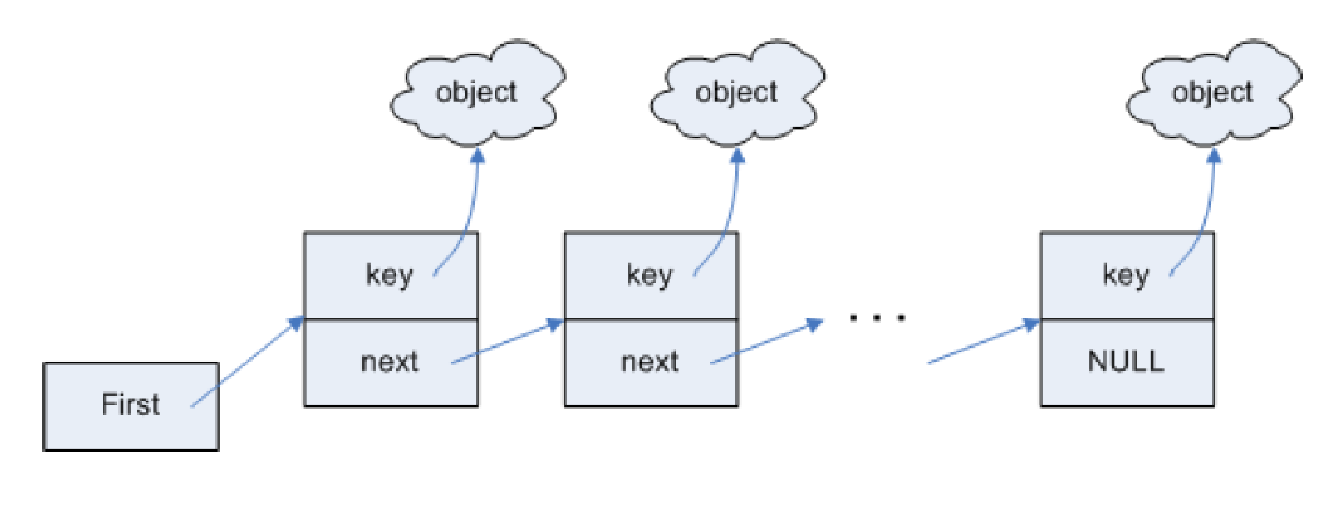
\includegraphics[width=1\linewidth]{1}}
\caption{Структура линейного односвязного списка.}
\end{figure}